\documentclass[noend]{amsproc}

\renewcommand{\arraystretch}{1.3}
\linespread{1}

\usepackage{amsthm,amsmath,amsfonts,mathrsfs,amssymb,lscape,array}
\usepackage{algorithm}
\usepackage{algorithmic}
\usepackage{multirow}
\usepackage{rotating}
\usepackage{enumerate}
\usepackage{enumitem}
\usepackage{natbib}
\usepackage{url}
\usepackage{calc}

\newtheorem{theorem}{Theorem}
\newtheorem{defn}[theorem]{Definition}
\newtheorem{lemma}[theorem]{Lemma}
\theoremstyle{definition}
\newtheorem{remark}[theorem]{Remark}
\newtheorem{example}[theorem]{Example}

% ALGORITHM style
\renewcommand{\algorithmicrequire}{\textbf{Input:}}
\renewcommand{\algorithmicensure}{\textbf{Output:}}

% fix spacing at \left and \right, see
% http://tex.stackexchange.com/questions/2607/spacing-around-left-and-right
\let\originalleft\left
\let\originalright\right
\renewcommand{\left}{\mathopen{}\mathclose\bgroup\originalleft}
\renewcommand{\right}{\aftergroup\egroup\originalright}

\newcommand{\myunderbrace}[3]{%
\makebox[\minof{0pt}{\widthof{$#1$}/2-\widthof{$#2$}/2-\widthof{$#3$}}]{}%
\underbrace{#1}_{\displaystyle\phantom{#3}#2 #3}}

\newcommand{\Singular}{\textsc{Singular}}
\newcommand{\realclassify}{\texttt{realclassify.lib}}
\newcommand{\tY}{\widetilde{Y}}

\DeclareMathOperator{\ord}{ord}
\DeclareMathOperator{\requiv}{\overset{r}{\sim}}
\DeclareMathOperator{\csim}{\mathrel{\smash{\overset{\C}{\sim}}}}
\DeclareMathOperator{\rsim}{\mathrel{\smash{\overset{\R}{\sim}}}}
\DeclareMathOperator{\ksim}{\mathrel{\smash{\overset{\K}{\sim}}}}
\DeclareMathOperator{\m}{\mathfrak{m}}
\DeclareMathOperator{\jt}{jet}
\DeclareMathOperator{\supp}{supp}
\DeclareMathOperator{\sign}{sign}
\DeclareMathOperator{\N}{\mathbb{N}}
\DeclareMathOperator{\Z}{\mathbb{Z}}
\DeclareMathOperator{\Q}{\mathbb{Q}}
\DeclareMathOperator{\R}{\mathbb{R}}
\DeclareMathOperator{\C}{\mathbb{C}}
\DeclareMathOperator{\K}{\mathbb{K}}
\DeclareMathOperator{\A}{\mathbb{A}}
\DeclareMathOperator{\NF}{NF}
\DeclareMathOperator{\T}{T}
\DeclareMathOperator{\Aut}{Aut}
\DeclareMathOperator{\id}{id}
\DeclareMathOperator{\Quot}{Quot}
\DeclareMathOperator{\dash}{\!\textnormal{-}\!}
\DeclareMathOperator{\jet}{jet}
\usepackage{tikz}
\usetikzlibrary{matrix,arrows}

\hyphenation{equiva-lence}
\hyphenation{ne-ces-sary}

\title[The Classification of Real Singularities Using \textsc{Singular}, %
Part II]%
{The Classification of Real Singularities Using \textsc{Singular}\\
Part II: The Structure of the Equivalence Classes of the Unimodal %
Singularities}

\author{Magdaleen S. Marais}
\address{Magdaleen S. Marais\\
African Institute for Mathematical Sciences and Stellenbosch University\\
6 Melrose Rd\\
Muizenberg 7945, Cape Town\\
South Africa}
\email{magdaleen@aims.ac.za}

\author{Andreas Steenpa\ss}
\address{Andreas Steenpa\ss\\
Department of Mathematics\\
University of Kaiserslautern\\
Erwin-Schr\"odinger-Str.\\
67663 Kaiserslautern\\
Germany}
\email{steenpass@mathematik.uni-kl.de}

\thanks{ }
\subjclass[2000]{}
\keywords{}
\begin{document}
\begin{abstract}
The algorithms implemented in the library ``realclassify.lib" in
\textsc{singular} are discussed in this paper. The purpose of this library is
to classify the~$0$ and $1$ modal isolated hypersurface singularities at $0$ of
corank $0$, $1$ and $2$ over the real numbers as computed by \citet{AVG1985}.
\end{abstract}
\maketitle


\section{Introduction}

\begin{table}[tp]
\centering
\caption{Normal forms of singularities of modality $1$ and corank $2$}
\label{tab:normal_forms}
\begin{tabular}{|c|c|c|c|c|}
\hline

\multicolumn{1}{|c}{}
 & & Complex     & Normal forms     & \multirow{2}{*}{Restrictions} \\
\multicolumn{1}{|c}{}
 & & normal form & of real subtypes &                               \\
\hline\hline


\multirow{6}{*}{\begin{sideways}Parabolic\end{sideways}}

& \multirow{4}{*}{$X_9$} & \multirow{4}{*}{$x^4+ax^2y^2+y^4$}
  & $+x^4+ax^2y^2+y^4$ $(X_9^{++})$ & \multirow{2}{*}{$a^2\neq4$} \\\cline{4-4}
&&& $-x^4+ax^2y^2-y^4$ $(X_9^{--})$ &                             \\\cline{4-5}
&&& $+x^4+ax^2y^2-y^4$ $(X_9^{+-})$ & \multirow{2}{*}{$a^2\neq-4$}\\\cline{4-4}
&&& $-x^4+ax^2y^2+y^4$ $(X_9^{-+})$ &                             \\\cline{2-5}

& \multirow{2}{*}{$J_{10}$} & \multirow{2}{*}{$x^3+ax^2y^2+xy^4$}
  & $x^3+ax^2y^2+xy^4$ $(J_{10}^+)$ & $a^2 \neq 4$ \\ \cline{4-5}
&&& $x^3+ax^2y^2-xy^4$ $(J_{10}^-)$ & -            \\ \hline


\multirow{12}{*}{\begin{sideways}Hyperbolic\end{sideways}}

& \multirow{2}{*}{$J_{10+k}$} & \multirow{2}{*}{$x^3+x^2y^2+ay^{6+k}$}
  & $x^3+x^2y^2+ay^{6+k}$ $(J_{10+k}^+)$
      & \multirow{2}{*}{$a \neq 0,\; k > 0$} \\ \cline{4-4}
&&& $x^3-x^2y^2+ay^{6+k}$ $(J_{10+k}^-)$ &   \\ \cline{2-5}

& \multirow{4}{*}{$X_{9+k}$} & \multirow{4}{*}{$x^4+x^2y^2+ay^{4+k}$}
  & $+x^4+x^2y^2+ay^{4+k}$ $(X_{9+k}^{++})$
      & \multirow{4}{*}{$a \neq 0,\; k > 0$}  \\ \cline{4-4}
&&& $-x^4-x^2y^2+ay^{4+k}$ $(X_{9+k}^{--})$ & \\ \cline{4-4}
&&& $+x^4-x^2y^2+ay^{4+k}$ $(X_{9+k}^{+-})$ & \\ \cline{4-4}
&&& $-x^4+x^2y^2+ay^{4+k}$ $(X_{9+k}^{-+})$ & \\ \cline{2-5}

& \multirow{4}{*}{$Y_{r,s}$} & \multirow{4}{*}{$x^2y^2+x^r+ay^s$}
  & $+x^2y^2+x^r+ay^s$ $(Y_{r,s}^{++})$
      & \multirow{4}{*}{$a \neq 0,\; r,s > 4$} \\ \cline{4-4}
&&& $-x^2y^2-x^r+ay^s$ $(Y_{r,s}^{--})$ &      \\ \cline{4-4}
&&& $+x^2y^2-x^r+ay^s$ $(Y_{r,s}^{+-})$ &      \\ \cline{4-4}
&&& $-x^2y^2+x^r+ay^s$ $(Y_{r,s}^{-+})$ &      \\ \cline{2-5}

& \multirow{2}{*}{$\tY_r$} & \multirow{2}{*}{$(x^2+y^2)^2+ax^r$}
  & $+(x^2+y^2)^2+ax^r$ $(\tY_r^+)$
      & \multirow{2}{*}{$a \neq 0,\; r > 4$} \\ \cline{4-4}
&&& $-(x^2+y^2)^2+ax^r$ $(\tY_r^-)$ &        \\ \hline


\multirow{12}{*}{\begin{sideways}Exceptional\end{sideways}}

& $E_{12}$ & $x^3+y^7+axy^5$ & $x^3+y^7+axy^5$ & - \\ \cline{2-5}

& $E_{13}$ & $x^3+xy^5+ay^8$ & $x^3+xy^5+ay^8$ & - \\ \cline{2-5}

& \multirow{2}{*}{$E_{14}$} & \multirow{2}{*}{$x^3+y^8+axy^6$}
  & $x^3+y^8+axy^6$ $(E_{14}^+)$ & \multirow{2}{*}{-} \\ \cline{4-4}
&&& $x^3-y^8+axy^6$ $(E_{14}^-)$ &                    \\ \cline{2-5}

& $Z_{11}$ & $x^3y+y^5+axy^4$ & $x^3y+y^5+axy^4$ & - \\ \cline{2-5}

& $Z_{12}$ & $x^3y+xy^4+ax^2y^3$ & $x^3y+xy^4+ax^2y^3$ & - \\ \cline{2-5}

& \multirow{2}{*}{$Z_{13}$} & \multirow{2}{*}{$x^3y+y^6+axy^5$}
  & $x^3y+y^6+axy^5$ $(Z_{13}^+)$ & \multirow{2}{*}{-} \\ \cline{4-4}
&&& $x^3y-y^6+axy^5$ $(Z_{13}^-)$ &                    \\ \cline{2-5}

& \multirow{2}{*}{$W_{12}$} & \multirow{2}{*}{$x^4+y^5+ax^2y^3$}
  & $+x^4+y^5+ax^2y^3$ $(W_{12}^+)$ & \multirow{2}{*}{-} \\ \cline{4-4}
&&& $-x^4+y^5+ax^2y^3$ $(W_{12}^-)$ &                    \\ \cline{2-5}

& \multirow{2}{*}{$W_{13}$} & \multirow{2}{*}{$x^4+xy^4+ay^6$}
  & $+x^4+xy^4+ay^6$ $(W_{13}^+)$ & \multirow{2}{*}{-} \\ \cline{4-4}
&&& $-x^4+xy^4+ay^6$ $(W_{13}^-)$ &                    \\ \hline

\end{tabular}
\end{table}


\section{The Sets of Parameter Transformations
$\boldsymbol{P_1}$, $\boldsymbol{P_2}$, and $\boldsymbol{P_3}$}

For the unimodal singularities, we add the value of the parameter which occurs
in the normal form as given in Table~\ref{tab:normal_forms} in parentheses to
the name of the singularity (sub-)type if we want to refer specifically to the
corresponding equivalence class. For instance, we denote by $E_{14}(3)$ the
(complex or real) right-equivalence class of $x^3+y^8+3xy^6$.

For any specific equivalence class $T$, we denote by $\NF(T)$ its normal form
as shown in Table~\ref{tab:normal_forms}, i.e.\@ we write
$\NF\left(E_{14}(a)\right) = \NF\left(E_{14}^+(a)\right)$ for the polynomial
$x^3+y^8+axy^6$ and $\NF\left(E_{14}^-(a)\right)$ for $x^3-y^8+axy^6$.

Throughout the rest of this article, let $\K$ be, in each case, either $\R$ or
$\C$.

\begin{defn}
Let $S \subset \Aut_{\K}(\K[[x_1,\ldots,x_n]])$ be a subset of the set of
$\K$-algebra automorphisms of $\K[[x_1, \ldots, x_n]]$ and let
$f, g \in \K[[x_1, \ldots, x_n]]$ be two power series.
\begin{enumerate}
\item We denote the set of all automorphisms in $S$ which take $f$ to $g$ by
$\T_{\K}^S(f,g)$, i.e.\@
\[
\T_{\K}^S(f,g):=\{\phi\in S\mid \phi(f)=g\}\,.
\]

\item If $S=\Aut_{\K}(\K[[x_1,\ldots,x_n]])$, we simply write
$\T_{\K}(f,g)$ for $\T_{\K}^S(f,g)$, i.e.\@
\[
\T_{\K}(f,g)
:= \{\phi \in \Aut_{\K}(\K[[x_1, \ldots, x_n]]) \mid \phi(f) = g \} \,.
\]

\item $f$ and $g$ are called $\K$-equivalent, denoted by
$f \ksim g$, if $\T_{\K}(f,g) \neq \varnothing$.
\end{enumerate}
\end{defn}

The above definition is the key ingredient for the definition of $P_1$, $P_2$,
and $P_3$. We also need the following notation.

\begin{remark}
As usual, we denote the quotient field
$\Quot(\K[a])$ by $\K(a)$. Let $f \in \K(a)[[x_1,\ldots,x_n]]$ be a power
series over this quotient field. Then $f$ can be written as
$f = \sum_{\nu \in \N^n} c_\nu \boldsymbol{x}^\nu$ with coeffients
$c_\nu = \frac{p_\nu}{q_\nu} \in \K(a)$ where $p_\nu, q_\nu \in \K[a]$ are
polynomials of minimal degree with this property and $q_\nu \neq 0$ for all
$\nu \in \N^n$.

If we consider the polynomials $p_\nu, q_\nu$ as polynomial functions
$p_\nu, q_\nu: \; \K \rightarrow \K$, then we may also consider the
coefficients $c_\nu$ as functions
$c_\nu: \; \K \setminus V(q_\nu) \rightarrow \K$ where $V(q_\nu)$ is the set of
points where $q_\nu$ vanishes. Via this correspondence, we finally get power
series
$f(u) := \sum_{\nu \in \N^n} c_\nu(u) \boldsymbol{x}^\nu
\in \K[[x_1,\ldots,x_n]]$ for each value
$u \in \K \setminus \bigcup_{\nu \in \N^n} V(q_\nu)$.

We will use the notation $f(u)$ throughout this paper. Note that it is
compatible with the notations for equivalence classes and normal forms of
unimodal singularities introduced above in the sense that, e.g.,
$\NF(E_{14}(a))(b) = \NF(E_{14}(b))$.
\end{remark}

We can now state the main definition of this section.

\begin{defn}
\leavevmode
\begin{enumerate}
\item
Given power series $f,g \in \C(a)[[x_1,\ldots,x_n]]$, we define the
first set of parameter transformations of $f$ and $g$ as
\begin{align*}
P_1(f, g)
:= \{ (u, v) \in \C^2 \mid
&f(u) \text{ and } g(v) \text{ are well-defined and } \\
&\T_{\C}(f(u), g(v)) \neq \varnothing \} \,.
\end{align*}

\item
Given power series $f,g \in \R(a)[[x_1,\ldots,x_n]]$, we define the
second set of parameter transformations of $f$ and $g$ as
\begin{align*}
P_2(f, g)
:= \{ (u, v) \in \R^2 \mid
&f(u) \text{ and } g(v) \text{ are well-defined and } \\
&\T_{\C}(f(u), g(v)) \neq \varnothing \} \,.
\end{align*}

\item
Given power series $f,g \in \R(a)[[x_1,\ldots,x_n]]$, we define the
third set of parameter transformations of $f$ and $g$ as
\begin{align*}
P_3(f, g)
:= \{ (u, v) \in \R^2 \mid
&f(u) \text{ and } g(v) \text{ are well-defined and } \\
&\T_{\R}(f(u), g(v)) \neq \varnothing \} \,.
\end{align*}
\end{enumerate}
\end{defn}

\begin{remark}
\leavevmode
\begin{enumerate}
\item
Note that we have $P_3(f, g) \subseteq P_2(f, g) \subseteq P_1(f, g)$ for any
two power series $f,g \in \R(a)[[x_1,\ldots,x_n]]$.

\item
For any two unimodal singularity (sub-)types $T_1, T_2$, we simply write
$P_i(T_1,T_2)$ instead of $P_i(\NF(T_1(a)), \NF(T_2(a)))$, e.g., we write
$P_1(E_{14}, E_{14})$ for $P_1(\NF(E_{14}(a)), \NF(E_{14}(a)))$.
\end{enumerate}
\end{remark}

For the parabolic singularity types $X_9$ and $J_{10}$, the sets $P_1$, $P_2$,
and $P_3$ can be described in terms of the following definition.

\begin{defn}
For $\Omega \subset \C$, let $(f_i: \Omega \rightarrow \C)_{i \in I}$ be a
family of complex-valued functions on $\Omega$. We define the joint graph of
$(f_i)_{i \in I}$ over $\Omega$ as
\[
\Gamma_\Omega((f_i)_{i \in I})
:= \{ (a, f_i(a)) \in \Omega \times \C \mid a\in \Omega,\; i \in I \}\,.
\]
\end{defn}

It turns out that for the hyperbolic and exceptional unimodal singularities,
$P_1$, $P_2$ and $P_3$ are just unions of sets of the form $(a, ra)_{a \in \K}$
for some $r \in \K$. For those cases we use the following notations.

\begin{defn}
For any polynomial $p(X) \in \C[X]$, we define the sets $C(p(X))$ and $R(p(X))$
as
\begin{align*}
C(p(X)) &:= \{ (a, ra) \in \C^2 \mid a, r \in \C, \; p(r) = 0 \} \,, \\
R(p(X)) &:= \{ (a, ra) \in \R^2 \mid a, r \in \R, \; p(r) = 0 \} \,.
\end{align*}
\end{defn}


\section{Weighted Jets and Filtrations of Power Series and Transformations}

We briefly introduce the concepts of (piecewise) weighted jets and filtrations.
For background regarding the definitions in this section, we refer to
\citet{A1974}. We assume that the reader is familiar with the notions of
weighted degrees, quasihomogeneous polynomials, and Newton polygons.

\begin{remark}
Let $w$ be a weight on the variables $(x_1, \ldots, x_n)$. Throughout this
paper we always assume that the weighted degree of $x_i$, denoted by
$w\dash\deg(x_i)$, is a natural number for each $i = 1, \ldots, n$.
\end{remark}

\begin{defn}
Let $w_0 := (w_1, \ldots, w_s) \in \left(\N^n\right)^s$ be a finite family of
weights on the variables $(x_1, \ldots, x_n)$. For any monomial
$m \in \K[x_1,\ldots,x_n]$, we define the piecewise weight of $m$ w.r.t.\@
$w_0$ as
\[
w_0\dash\deg(m) := \min_{i = 1, \ldots, s} w_i\dash\deg(m) \,.
\]
A polynomial $f \in \K[x_1,\ldots,x_n]$ is called piecewise quasihomogeneous
w.r.t.\@ $w_0$ if $w_0\dash\deg(t_1) = w_0\dash\deg(t_2)$ for any two terms
$t_1, t_2$ of $f$.
\end{defn}

\begin{defn}
Let $w$ be a (piecewise) weight on the variables $(x_1,\ldots,x_n)$.

\begin{enumerate}
\item
Let $f = \sum_{i = 0}^{\infty} f_{i,w}$ be the decomposition of
$f \in \K[[x_1,\ldots,x_n]]$ into weighted homogeneous parts $f_{i,w}$ of
$w$-degree $i$. We denote the weighted $j$-jet of $f$ w.r.t.\@ $w$ by
\[
w \dash \jet(f, j) := \sum_{i = 0}^j f_{i,w} \,.
\]

\item
A power series in $\K[[x_1,\ldots,x_n]]$ has filtration $d \in \N$ if all its
monomials are of weighted degree $d$ or higher. The power series of filtration
$d$ form a vector space $E_d^w \subset \K[[x_1,\ldots,x_n]]$.
\end{enumerate}
\end{defn}

\begin{remark}
Note that $d < d'$ implies $E_{d'}^w \subseteq E_d^w$. Since the filtration of
the product $E_{d'}^w \cdot E_d^w$ is $d'+d$, it follows that $E_d^w$ is an
ideal in the ring of power series. We denote the ideal consisting of power
series of filtration strictly greater than $d$ by $E_{>d}^w$. If the weight
of each variable is $1$, we simply write $E_d$ and $E_{>d}$, respectively.
\end{remark}

There are also similar concepts for coordinate transformations:

\begin{defn}\label{def:jet_phi}
Let $\phi$ be a $\K$-algebra automorphism of $\K[[x_1,\ldots,x_n]]$ and let
$w$ be a (piecewise) weight on the variables.

\begin{enumerate}
\item
For $j > 0$ we define the weighted $j$-jet of $\phi$ w.r.t.\@ $w$, denoted by
$\phi_j^w$, to be the automorphism given by
\[
\phi_j^w(x_i) := w\dash\jet(\phi(x_i),w\dash\deg(x_i)+j) \quad
\forall i = 1,\ldots,n \,.
\]
If the weight of each variable is $1$, i.e.\@ $w = (1, \ldots, 1)$, we simply
write $\phi_j$ for $\phi_j^w$.

\item\label{enum:filtration}
$\phi$ has filtration $d$ if, for all $\lambda \in \N$,
\[
(\phi-\id)E_\lambda^w \subset E_{\lambda+d}^w \,.
\]
\end{enumerate}
\end{defn}

\begin{remark}\label{rem:weighted_jet}
Let $\phi$ be a $\K$-algebra automorphism of $\K[[x_1,\ldots,x_n]]$.

\begin{enumerate}
\item
Note that $\phi_0(x_i) = \jet(\phi(x_i), 1)$ for all $i = 1, \ldots, n$.
Furthermore note that $\phi_0^w$ may have filtration less than or equal to $0$
for any weight $w$.

\item\label{enum:weighted_jet}
Let $w_0 = (w_1, \ldots, w_s) \in \left(\N^n\right)^s$ be a piecewise weight on
$(x_1, \ldots, x_n)$ and let $f_0 \in \K[x_1,\ldots,x_n]$ be piecewise
quasihomogeneous of degree $d_0$ w.r.t.\@ $w_0$ and
$f_1 \in \K[x_1,\ldots,x_n]$ quasihomogeneous of degree $d_1$ w.r.t.\@
$w_1$. We always have
$(\phi-\phi_\delta^{w_1})(f_1) \in E_{>d_1+\delta}^{w_1}$, but the analogon for
$w_0$ does not hold in general: To give a counterexample, let us consider the
case $n = s = 2$, $w_0 = ((1,4), (4,1))$, $f_0 = x_1 x_2$, and let $\phi$ be
given by $\phi(x_1) := x_1+x_2^2$, $\phi(x_2) := x_2+x_2^2$. Then $f_0$ is of
degree $d_0 = 5$, but $(\phi-\phi_0^{w_0})(f_0) = x_2^4$ is of degree $4$
w.r.t.\@ $w_0$ and thus not an element of $E_5^{w_0} = E_{d_0+0}^{w_0}$.
\end{enumerate}
\end{remark}


\section{Sufficient Sets of Transformations Between Real Normal Forms}

The results in this section considerably narrow down the transformations we
need to consider between specific unimodal normal forms of the same main type
in order to determine equivalence. In fact these results are in many cases the
main step for determining the structure of the equivalence classes of the
unimodal singularities up to corank $2$.

\begin{defn}
Let $f$ and $g$ be elements in $\C(a)[[x_1,\ldots,x_n]]$ and let $S$ be a
subset of $\Aut_{\C}(\C[[x_1,\ldots,x_n]])$. We call $S$ a sufficient set of
coordinate transformations for $f$ and $g$ if
\[
\forall u,v \in \C: \quad
\left(T_{\C}(f(u),g(v)) \neq \varnothing
\;\Leftrightarrow\; \T_{\C}^S(f(u),g(v)) \neq \varnothing\right) \,.
\]
\end{defn}

The sufficient sets which we consider here can be described using the
following notation.

\begin{defn}
Let $M_x$ and $M_y$ be sets of monomials in $\C[[x,y]]$ and let $\C\! M_x$ and
$\C\! M_y$ be the $\C$-vector spaces spanned by these sets, i.e.\@
$\C\! M_x := \bigoplus_{m \in M_x} \C \cdot m$ and analogously for $\C\! M_y$. 
We define the set of coordinate transformations spanned by $M_x$ and $M_y$ as
\[
S(M_x, M_y) := \{ \phi \in \Aut_{\C}(\C[[x,y]]) \mid
\phi(x) \in \C\! M_x,\; \phi(y) \in \C\! M_y \} \,.
\]
\end{defn}

\begin{theorem}\label{thm:sufficient_sets}
Let $T$ be one of the main singularity types listed in
Table~\ref{tab:sufficient_sets}, let $M_x$ and $M_y$ be the corresponding sets
of monomials, and let $T_1$ and $T_2$ be subtypes of $T$. Then $S(M_x, M_y)$
is a sufficient set of coordinate transformations for $\NF(T_1)$
and $\NF(T_2)$.

\begin{table}[htb]
\centering
\caption{Sufficient sets for some unimodal singularities}
\label{tab:sufficient_sets}
\begin{tabular}{|c|c|c|c|}
\hline

& $T$ & $M_x$ & $M_y$ \\
\hline\hline


\multirow{2}{*}{\begin{sideways}P.\end{sideways}}

& $X_9$    & $\{x, y\}$   & $\{x, y\}$ \\ \cline{2-4}
& $J_{10}$ & $\{x, y^2\}$ & $\{y\}$    \\ \hline


\multirow{3}{*}{\begin{sideways}Hyperb.\end{sideways}}

& $J_{10+k}$ & $\{x\}$    & $\{y\}$    \\ \cline{2-4}
& $X_{9+k}$  & $\{x\}$    & $\{y\}$    \\ \cline{2-4}
& $Y_{r,s}$  & $\{x, y\}$ & $\{x, y\}$ \\ \hline


\multirow{3}{*}{\begin{sideways}Except.\end{sideways}}

& $E_{12}, E_{13}, E_{14}$ & $\{x\}$ & $\{y\}$ \\ \cline{2-4}
& $Z_{11}, Z_{12}, Z_{13}$ & $\{x\}$ & $\{y\}$ \\ \cline{2-4}
& $W_{12}, W_{13}$         & $\{x\}$ & $\{y\}$ \\ \hline

\end{tabular}
\end{table}

\end{theorem}

\begin{proof}
We give different proofs for the parabolic, the hyperbolic, and the exceptional
cases as indicated in Table~\ref{tab:sufficient_sets}.

In each case, let $T_1$ and $T_2$ be subtypes of the same main type $T$, and
for $u \in \C$ let $\phi \in \Aut_{\C}(\C[[x,y]])$ be a coordinate
transformation which takes $f := \NF(T_1(u))$ to $\NF(T_2(v))$ for some
$v \in \C$.

\begin{description}[font=\normalfont\itshape,%
leftmargin=0cm,labelindent=\parindent]

\item[Parabolic cases]
The normal forms of both $X_9$ and $J_{10}$ are
quasihomogeneous with weights $w := (1,1)$ and $w := (2,1)$, respectively. Let
us first consider the case $T = X_9$. We have
\[
\phi(f) = \phi_0^w(f)+(\phi-\phi_0^w)(f) = \phi_0^w(f)+R
\]
with $R \in E_{>4}^w$. This implies $\phi(f) = \phi_0^w(f)$ because
$\phi(f) = \NF(T_2(v))$ is homogeneous of degree $4$ w.r.t.\@ the weight $w$.
So any possible value of $v$ which can be obtained by some
$\phi \in \Aut_{\C}(\C[[x,y]])$ can also be reached via
$\phi_0^w \in S\left(\{x,y\}, \{x,y\}\right)$, i.e.\@,
$S\left(\{x,y\}, \{x,y\}\right)$ is a sufficient set of coordinate
transformations for $\NF(T_1)$ and $\NF(T_2)$.

Let us now consider the case $T = J_{10}$.
Again we have $\phi(f) = \phi_0^w(f)$, but
in this case
$\phi_0^w$ is of the form
$\phi_0^w(x) = \alpha x + \beta y + \gamma y^2$,
$\phi_0^w(y) = \delta y$ with
$\alpha, \beta, \gamma, \delta \in \C$. Comparing the coefficients of
$\phi(f) = \NF(T_2(v))$ and
$\phi_0^w(f) = \beta^3 y^3 + (\text{other terms})$ yields
$\beta = 0$ and therefore $\phi_0^w \in S(\{x, y^2\}, \{y\})$
as expected.

\item[Hyperbolic cases]
We present a proof for the main type $T = J_{10+k}$, the proofs for $X_{9+k}$
and $Y_{r,s}$ are similar. It does not matter for the arguments which follow
whether we assume $T_1 = J_{10+k}^-$ or $T_1 = J_{10+k}^-$, the same holds for
$T_2$. We write $\pm$ whenever the sign can be either plus or minus in order to
prove all cases at once.

The Newton polygon of $f = \NF(T_1(u)) = x^3 \pm x^2 y^2 + uy^{6+k}$ has two
faces defined by $f_1 := x^3 \pm x^2 y^2$ and $f_2 := \pm x^2 y^2 + uy^{6+k}$.
Let $w_0$ be the piecewise weight given by the two weights
$w_1 := (12+2k, 6+k)$ and $w_2 := (12+3k, 6)$. Then $f$ is piecewise
quasihomogeneous of degree $d := 36+6k$ w.r.t.\@ $w_0$.

We now proceed in three steps: In the first two, we show
$\phi_0^{w_1} \in S(\{x\}, \{y\})$ and $\phi_0^{w_2} \in S(\{x\}, \{y\})$.
Finally we conclude that $\phi(f)$ is equal to $\phi_0^{w_0}(f)$ and that
$\phi_0^{w_0}$ is an element of $S(\{x\}, \{y\})$ which proves the claim.

The transformation $\phi_0^{w_1}$ is generically of the form
$\phi_0^{w_1}(x) = \alpha x + \beta_1 y + \beta_2 y^2$,
$\phi_0^{w_1}(y) = \gamma y$ with $\alpha, \beta_1, \beta_2, \gamma \in \C$ and
$\alpha, \gamma \neq 0$. With these notations we have
\begin{align*}
\phi(f)
&= \phi_0^{w_1}(f) + (\phi-\phi_0^{w_1})(f) \\
&= \beta_1^3 y^3 + (3\alpha\beta_2^2 \pm 2\alpha\beta_2\gamma^2) xy^4
+ (\beta_2^3 \pm \beta_2^2\gamma^2) y^6 + (\text{other terms})
\end{align*}
on the one hand and
\begin{align*}
\phi(f)
&= \NF(T_1(v)) \\
&= x^3 \pm x^2 y^2 + vy^{6+k}
\end{align*}
on the other hand. This implies $\beta_1 = \beta_2 = 0$ and hence
$\phi_0^{w_1} \in S(\{x\}, \{y\})$.

The second step is a proof by contradiction. Let $m$ be the largest integer
which is not greater than $\frac{k}{2}+2$. Then similar as above, the
automorphism $\phi_0^{w_2}$ is of the form
\begin{align*}
\phi_0^{w_2}(x)
&= \alpha x + \beta_1 y + \beta_2 y^2 + \ldots + \beta_m y^m \,, \\
\phi_0^{w_2}(y) &= \gamma y
\end{align*}
with $\alpha, \beta_1, \ldots, \beta_m, \gamma \in \C$ and
$\alpha, \gamma \neq 0$. We have already shown $\beta_1 = \beta_2 = 0$. Assume
$\beta_s \neq 0$ for some $s \in \{3, \ldots, m\}$ and let $s$ be minimal with
this property. Then the coefficient of $xy^{s+2}$ in
$\phi(f) = \phi_0^{w_2}(f) + (\phi-\phi_0^{w_2})(f)$ is $\pm 2\beta_s$ which
implies $\beta_s = 0$ in contradiction to the assumption. Hence
$\beta_3 = \ldots = \beta_m = 0$ and $\phi_0^{w_2} \in S(\{x\}, \{y\})$.

For the last step, we consider the following equations:
\begin{align*}
\phi(f) &= \phi_0^{w_1}(f)
+\myunderbrace{(\phi-\phi_0^{w_1})(f)}{=}{: R_1 \in E_{>d}^{w_1}} \\[1ex]
\phi(f) &= \phi_0^{w_2}(f)
+\myunderbrace{(\phi-\phi_0^{w_2})(f)}{=}{: R_2 \in E_{>d}^{w_2}} \\[1ex]
\phi(f) &= \phi_0^{w_0}(f)
+\myunderbrace{(\phi-\phi_0^{w_0})(f)}{=}{: R_0}
\end{align*}
Note that it is not a priori clear that $R_0$ lies in $E_{>d}^{w_0}$ if we only
consider these equations, cf.\@
Remark~\ref{rem:weighted_jet}(\ref{enum:weighted_jet}). Nevertheless, this can
be shown if we take into account the results of the two previous steps: By
definition of the piecewise weight $w_0$, any term in $\phi_0^{w_0}(x)$ also
appears in $\phi_0^{w_1}(x)$ or $\phi_0^{w_2}(x)$ (or both), analogously for
$\phi_0^{w_0}(y)$. Therefore we have $\phi_0^{w_0}(x) = \alpha x$ and
$\phi_0^{w_0}(y) = \gamma y$, hence
$\phi_0^{w_0} = \phi_0^{w_1} = \phi_0^{w_2}$ and
$\phi_0^{w_0} \in S(\{x\}, \{y\})$. This implies
\[
R_0 = R_1 = R_2 \in E_{>d}^{w_1} \cap E_{>d}^{w_2} = E_{>d}^{w_0} \,.
\]
Since $\phi(f) = \NF(T_2(v))$ is piecewise quasihomogeneous of degree $d$
w.r.t.\@ $w_0$, we finally get $R_0 = 0$ and $\phi(f) = \phi_0^{w_0}(f)$. This
proves the claim.

\item[Exceptional cases]
The normal forms of all the exceptional cases in
Table~\ref{tab:sufficient_sets} are semi-quasihomogeneous polynomials, i.e., in
these cases $f = \NF(T_1(u))$ is of the form $f = f_0+f_1$ where $f_0$ is
quasihomogeneous of degree $d \in \N$ w.r.t.\@ some weight $w = (w_x, w_y)$,
$f_1$ has weighted degree $d+\delta > d$, and the Milnor number $\mu(f_0)$ of
$f_0$ is finite \citep[for the definition of the Milnor number, see][]{MS2013}.
In all the cases, $f_1$ consists of the term which contains the parameter and
we have
\begin{align*}
\phi(f) &= \phi_\delta^w(f_0) + \phi_0^w(f_1)
+ \left(\phi-\phi_\delta^w\right)(f_0) + \left(\phi-\phi_0^w\right)(f_1) \\
&= w\dash\jet(\phi_\delta^w(f_0), d+\delta) + \phi_0^w(f_1) + R
\end{align*}
with $R \in E_{>d+\delta}^w$. As above, $\phi(f) = \NF(T_2(v))$ implies
$R = 0$. If we show
\begin{align}
\phi_\delta^w \in S\left(\{x\}, \{y\}\right) \,, \tag{$\ast$}
\end{align}
then it follows that $\phi_\delta^w$ is equal to $\phi_0^w$ and therefore
\begin{align*}
\phi(f)
&= w\dash\jet(\phi_0^w(f_0), d+\delta) + \phi_0^w(f_1) \\
&= \phi_0^w(f_0)+\phi_0^w(f_1) \\
&= \phi_\delta^w(f) \,.
\end{align*}
This, together with $(\ast)$, proves the claim.

The statement $(\ast)$ can be shown seperately for each of the eight cases by
some easy computations. We carry out the proof for $W_{13}$, the other cases
follow similarly. The normal forms of the subtypes of $W_{13}$ are
$\pm x^4+xy^4+ay^6$, so in this case we have $w = (4,3)$, $d = 16$, and
$\delta = 2$. The $\pm$-sign does not matter for the computations which follow,
but we carry it along in order to prove all subcases at once. The
transformation $\phi_\delta^w$ is generically of the form
\begin{align*}
\phi_\delta^w(x) &= \alpha x + \beta y + \gamma y^2 \,, \\
\phi_\delta^w(y) &= \delta y + \varepsilon x
\end{align*}
with $\alpha, \beta, \gamma, \delta, \varepsilon \in \C$ because any other term
would raise the weighted degree by more than $\delta$. With these notations, we
now successively compare the coefficients of
$w\dash\jet(\phi_\delta^w(f), d+\delta)$ and
$\phi(f) = \NF(T_2(v)) = \pm x^4+xy^4+vy^6$. The coefficient of $y^4$ in
$\phi_\delta^w(f)$ is $\pm \beta^4$ and therefore we have $\beta = 0$. The
remaining coefficients of $xy^4$, $x^2y^3$, and $x^3y^2$ are now
$\alpha\delta^4$, $4\alpha\delta^3\varepsilon$, and
$\pm 4\alpha^3\gamma+6\alpha\delta^2\varepsilon^2$, respectively, which shows
that (in this order) $\alpha\delta \neq 0$, $\varepsilon = 0$, and
$\gamma = 0$. Hence $\phi_\delta^w$ is in fact of the form
$\phi_\delta^w(x) = \alpha x$, $\phi_\delta^w(y) = \delta y$ which proves
$(\ast)$ for $T_1, T_2 \in \left\{W_{13}^+, W_{13}^-\right\}$.
\end{description}
\end{proof}


\section{On the Computation of the Results}\label{sec:computations}

Based on the previous section, the results presented in
Section~\ref{sec:results} can be computed using \Singular{} for all those
singularity types which are covered by Theorem~\ref{thm:sufficient_sets}. The
main tools for these computations are elimination, Gr\"obner covers, and
primary decomposition. For each pair of singularity subtypes~$T_1, T_2$, the
computation follows the same structure: One can first compute the set
$P_1(T_1, T_2)$ using elimination and factorization. The set $P_2(T_1, T_2)$
can then be derived from this as the intersection of $P_1(T_1, T_2)$ with
$\R \times \R$. In order to determine $P_3(T_1, T_2)$, one finally has to check
for each point or branch in $P_2(T_1, T_2)$ whether or not there is a real
transformation which changes the parameter in such a way. Gr\"obner covers and
primary decomposition are convenient tools to simplify the often complicated
ideals which occur in this last step.

Although our approach is almost algorithmic, we do not present it as an
algorithm here because each case requires slightly different means depending on
the intermediate results. Especially the computation of $P_3(T_1, T_2)$ is
rather straighforward in some cases whereas it requires careful considerations
in other cases.

However, writing down every detail of the computations for each case is beyond
the scope of this section. Instead, we will present the general framework and
give explicit \Singular{} commands for $T_1 = T_2 = X_9^{++}$ which is one of
the more complicated cases (cf. Theorem~\ref{thm:X9}).

The singularity type $\tY_r$ does not appear in Table~\ref{tab:sufficient_sets}
and thus needs special care. The structure of the equivalence classes of this
type can be computed on the basis of the data for the type $Y_{r,s}$, cf.\@
Section~\ref{ssec:Yr}.


\subsection{How to Compute $\boldsymbol{P_1(T_1, T_2)}$}%
\label{ssec:computing_P1}

Let $S \subset \Aut_{\C}(\C[[x,y]])$ be the sufficient set of
$\C[[x,y]]$-automorphisms for $T_1$ and $T_2$ given in
Theorem~\ref{thm:sufficient_sets}. Then $S$ can be covered by an automorphism
$\phi \in \Aut_{\C}(\C[[x,y]])$ with generic coefficients $t_1, \ldots, t_r$,
i.e.\@ by a $\phi$ of the form $\phi(x) = t_1 \cdot x + (\text{other terms})$
where for any element $\psi \in S$, one can plug in specific values for
$t_1, \ldots, t_r$ such that $\psi = \phi$.

Let us denote the parameter occurring in $T_1$ by $a$ and the one in $T_2$ by
$b$. By comparing the coefficients in $\phi(T_1(a))$ and $T_2(b)$, we get a set
of equations in $a, b, t_1, \ldots, t_r$ which is equivalent to
$\phi(T_1(a)) = T_2(b)$. Let $I \subset \C[a,b,t_1,\ldots,t_r]$ be the ideal
generated by these equations. Then the vanishing set $V(I)$ describes
completely which transformations take $T_1(a)$ to $T_2(b)$ for which values of
$a$ and $b$.

We can now eliminate the variables $t_1, \ldots, t_r$ from $I$ and thus obtain
an ideal $I' \subset \C[a,b]$ which is in all cases generated by one polynomial
$g$. This elimination geometrically corresponds to the projection
$\A_{\C}^{2+r} \supset V(I) \mapsto V(I') \subset \A_{\C}^2$. After factorizing
$g \in \C[a,b]$ into irreducible factors $g_1, \ldots, g_s$, we compute the
roots in $b$ of each factor (over $\C(a)$ or suitable extensions thereof if
necessary). We thus get roots of the form $b-f(a)$ where $f(a)$ can be
considered as a function in $a$. These functions explicitly determine the
possible values of $b$ for each given $a$ and their joint graph is exactly
$P_1(T_1, T_2)$.

\begin{example}\label{ex:P1}
We compute $P_1(X_9^{++}, X_9^{++})$ with Singular. For convenience we work
over $\Q(a,b,t_1,t_2,t_3,t_4)[x,y]$:
\begin{verbatim}
> ring R = (0,a,b,t1,t2,t3,t4), (x,y), dp;
> poly f = x^4+a*x^2*y^2+y^4;
\end{verbatim}
According to Theorem~\ref{thm:sufficient_sets},
\[
S = \{ \phi \in \Aut_{\C}(\C[[x,y]])
\mid \phi(x) = t_1 x + t_2 y,\; \phi(y) = t_3 x + t_4 y,\;
t_1, \ldots, t_4 \in \C \}
\]
is a sufficient set of automorphisms for $X_9$:
\begin{verbatim}
> map phi = R, t1*x+t2*y, t3*x+t4*y;
> matrix C = coef(phi(f), xy);
> print(C);
x^4,   x^3*y, x^2*y^2,x*y^3, y^4,  
C[2,1],C[2,2],C[2,3], C[2,4],C[2,5]
> C[2,1];
(a*t1^2*t3^2+t1^4+t3^4)
\end{verbatim}
Now the second row of the matrix \verb+C+ contains the coefficients of
$\verb+phi+(X_9^{++}(a))$, e.g.\@ \verb+C[2, 1]+ is the one belonging to $x^4$.
Using the corresponding coefficients of
$X_9^{++}(b) = x^4 + b \cdot x^2 y^2 + y^4$, we can define the ideal $I$ as
above:
\begin{verbatim}
> matrix D[1][5] = 1, 0, b, 0, 1;
> ideal I = C[2,1..5]-D[1,1..5];
\end{verbatim}
As the next step, we map this ideal to $\Q(a)[b,t_1,t_2,t_3,t_4]$ and eliminate
the variables~$t_i$:
\begin{verbatim}
> ring S = (0,a), (b,t1,t2,t3,t4), dp;
> ideal I = imap(R, I);
> ideal g = eliminate(I, t1*t2*t3*t4);
> g;
g[1]=(a^4-8*a^2+16)*b^6+(-a^6-720*a^2-1152)*b^4
+(8*a^6+720*a^4+20736)*b^2+(-16*a^6+1152*a^4-20736*a^2)
\end{verbatim}
Factorizing the single generator of this ideal finally yields the functions
$f_1^{1,1}, \ldots, f_6^{1,1}$ defined in Theorem~\ref{thm:X9}. Note that
$a^2 \neq 4$.
\begin{verbatim}
> factorize(g[1]);
[1]:
   _[1]=1
   _[2]=b+(-a)
   _[3]=b+(a)
   _[4]=(a-2)*b+(-2*a-12)
   _[5]=(a+2)*b+(-2*a+12)
   _[6]=(a+2)*b+(2*a-12)
   _[7]=(a-2)*b+(2*a+12)
[2]:
   1,1,1,1,1,1,1
\end{verbatim}
\end{example}


\subsection{How to Compute $\boldsymbol{P_2(T_1, T_2)}$}%
\label{ssec:computing_P2}

Given $P_1(T_1, T_2)$, it is easy to compute $P_2(T_1, T_2)$ even ``by hand''
because we have $P_2(T_1, T_2) = P_1(T_1, T_2) \cap (\R \times \R)$.

\begin{example}\label{ex:P2}
Continuing the example above, the values of
$f_1^{1,1}(a), \ldots, f_6^{1,1}(a)$ are clearly real for $a \in \R$, cf.\@
Theorem~\ref{thm:X9}. The set $P_2(X_9^{++}, X_9^{++})$ is thus the joint graph
of these functions over $\R \setminus \{-2, 2\}$.

To give another example, for $T_1 = T_2 = X_9^{+-}$ the set $P_1(T_1, T_2)$ is
the joint graph of $f_1^{i,i}, \ldots, f_6^{i,i}$ over
$\C \setminus \{-2i, 2i\}$. The values of $f_1^{i,i}(a)$ and $f_2^{i,i}(a)$ are
clearly real for $a \in \R$, but those of $f_2^{i,i}(a), \ldots, f_6^{i,i}(a)$
are not except at some exceptional points which are already covered by
$f_1^{i,i}$ and $f_2^{i,i}$. So in this case we have
\[
P_2(X_9^{+-}, X_9^{+-}) = \Gamma_{\R} \left(f_1^{i,i}, f_2^{i,i}\right)
= \Gamma_{\R} \left(f_1^{1,1}, f_2^{1,1}\right) \,.
\]
\end{example}


\subsection{How to Compute $\boldsymbol{P_3(T_1, T_2)}$}

Since $P_3(T_1, T_2) \subset P_2(T_1, T_2)$ by definition, we can determine
$P_3(T_1, T_2)$ by checking for each pair $(a,b) \in P_2(T_1, T_2)$ whether or
not there is a \emph{real} coordinate transformation
$\phi \in \Aut_{\R}(\R[[x,y]])$ which takes $T_1(a)$ to $T_2(b)$. This can be
reduced to a finite problem as follows: Let $g_j$, $j \in \{1,\ldots,s\}$, be
the irreducible factors of the polynomial $g$ as in
Section~\ref{ssec:computing_P1}. Then in all the cases, $P_2(T_1, T_2)$ is a
finite union of ``branches'' of the form $V(g_j)$ and some exceptional points.
We can check whether a branch $V(g_j)$ or an exceptional point $(q_a, q_b)$ in
$P_2(T_1, T_2)$ belongs $P_3(T_1, T_2)$ by simply adding appropriate relations
to the ideal~$I$ and looking at the real solutions of the resulting ideal. In
other words, we define $J := I+\langle g_j \rangle$ or
$J := I+\langle a-q_a, b-q_b \rangle$, respectively, and investigate
$V_{\R}(J)$. Note that we have $I \subset \R[a,b,t_1,\ldots,t_r]$ and
$g_j \in \R[a,b]$ and thus $J \subset \R[a,b,t_1,\ldots,t_r]$ in all the cases.

The set $P_3(T_1, T_2)$ is then the image of $V_{\R}(J) \subset \A_{\R}^{2+r}$
under the projection $\A_{\R}^{2+r} \rightarrow \A_{\R}^2$, i.e.\@ we have
$(p_a, p_b) \in P_3(T_1, T_2)$ if and only if there is a coordinate
transformation with real coefficients $(p_{t_1}, \ldots, p_{t_r})$ such that
$(p_a, p_b, p_{t_1}, \ldots, p_{t_r})$ is an element of
$V_{\R}(J) \subset \A_{\R}^{2+r}$.

It turns out that the ideal $J$ is quite complicated in some cases and that it
can be difficult to determine $V_{\R}(J)$ by just computing a Gr\"obner basis
of $J$. One way out is then to consider $J$ as a parametric ideal
$J \subset \R(a)[b,t_1,\ldots,t_r]$ and to compute a Gr\"obner cover thereof
by using the \Singular{} library \verb+grobcov.lib+ \citep{grobcov}.
A~Gr\"obner cover completely describes the possible shapes of Gr\"obner bases
of $J$ for different values of $a$. It contains a generic Gr\"obner basis of
$J$, i.e.\@ one which is a Gr\"obner basis except for finitely many exceptional
values of $a$, and additionally Gr\"obner bases of $J$ for each of these
exceptional values. The ideals in a Gr\"obner cover of $J$ typically have a
much easier structure then $J$ itself. We can thus treat them one by one and
determine their real solutions. We will often find generators such as
$(t_j)^4+1$, indicating that the vanishing set over $\R$ of this ideal is
empty.

If some of ideals in the Gr\"obner cover of $J$ are still to complicated and if
their vanishing set over $\R$ cannot be easily read off, another trick is to
compute a primary decomposition of these ideals with the \Singular{} library
\verb+primdec.lib+ \citep{primdec}. Typically, it is then easy to see that
some of the primary components have no solutions over $\R$ whereas the real
solutions of the remaining components can be easily determined.

\begin{example}
We have already seen in Example~\ref{ex:P2} that
$P_2(X_9^{++}, X_9^{++})$ is the joint graph of
$f_1^{1,1}, \ldots, f_6^{1,1}$ over $\R \setminus \{-2, 2\}$. We now have to
check for each of these functions whether their graph is also contained in
$P_3(X_9^{++}, X_9^{++})$.

This is clearly the case for $f_1^{1,1} = \id$. To check this for $f_3^{1,1}$,
we continue the \Singular{} session from Example~\ref{ex:P1}, add the
corresponding relation to the ideal $I$ and compute a Gr\"obner cover of the
resulting ideal $J$:
\begin{verbatim}
> ideal J = I, (a-2)*b+(-2*a-12);
> LIB "grobcov.lib";
> grobcov(J);
\end{verbatim}
The output of the last command is too long to be printed here. We will find
that the Gr\"obner basis of $J$ for generic $a$ contains the generators
$(t_2)^2+(t_4)^2$ and $(t_3)^2+(t_4)^2$ which imply $t_2 = t_3 = t_4 = 0$ for
any real solution of this ideal. But this is a contradiction to
$\verb+phi+ \in \Aut_{\R}(\R[[x,y]])$. The exceptional cases for the
parameter~$a$ are $a+2=0$, $a-2=0$, $a^2+12=0$, $a+6=0$, $a-6=0$, and $a=0$.
The first two cases are excluded by the definition of the equivalence class
$X_9^{++}$, $a^2+12=0$ would imply $a \not\in \R$, for $a+6=0$ and $a=0$ the
corresponding Gr\"obner bases of $J$ contain generators similar to those
mentioned above, and finally $a-6=0$ implies $b-6=0$ such that this case is
already covered by the graph of $f_1^{1,1}$.

To give one more example, let us consider $f_5^{1,1}$:
\begin{verbatim}
> J = I, (a+2)*b+(2*a-12);
> grobcov(J);
\end{verbatim}
The crucial generator of the Gr\"obner basis of $J$ for generic $a$ is now the
polynomial $(a+2)(t_4)^4-1$ which has a real root if and only if $a > -2$.
Considering the other generators, it is easy to see that given $t_4 \in \R$,
$t_1 = t_2 = t_3 = -t_4$ is a real solution. The exceptional values
of $a$ in this case are the same as above and again, we do not have to consider
$a+2=0$, $a-2=0$, and $a^2+12=0$. The relation $a+6=0$ implies $b+6=0$ which is
already covered by $f_1^{1,1}$. Finally,
$t_1 = t_2 = t_3 = \frac{1}{\sqrt[4]{2}}$, $t_4 = -\frac{1}{\sqrt[4]{2}}$ and
$t_1 = t_2 = t_3 = \frac{1}{\sqrt[4]{8}}$, $t_4 = -\frac{1}{\sqrt[4]{8}}$ are
real solutions for the cases $a=0$ and $a-6=0$, respectively. To sum up,
the graph of $f_5^{1,1}$ over $\R^{>-2}$ belongs to $P_3(X_9^{++}, X_9^{++})$,
but not the part over $\R^{<-2}$.

Continuing in this manner, one can show that $f_2^{1,1}$, $f_4^{1,1}$, and
$f_6^{1,1}$, do not contribute any additional points, so we get
\[
P_3(X_9^{++}, X_9^{++}) = \Gamma_{\R'} \left(f_1^{1,1}\right)
\cup \Gamma_{\R^{>-2}} \left(f_5^{1,1}\right)
\]
where $\R' := \R \setminus \{-2, 2\}$.
\end{example}

\begin{remark}
With the above notations, the irreducible factors $g_j$,
$j \in \{1,\ldots,s\}$, of the polynomial $g$ are luckily of degree $1$ in $b$
in almost all cases. If one of those factors, say $g_1$, has degree in $b$
greater than $1$, and if additionally the corresponding ideal $J = I + \langle
g_1 \rangle$ has both real and complex solutions, then an extra calculation is
needed: Let $f_1(a), \ldots, f_k(a)$ be the roots of $g_1$ in $b$ as above,
i.e.\@ $g_1 = (b-f_1(a)) \ldots (b-f_k(a))$ (over $\C(a)$ or over a suitable
extension thereof if necessary). Then we have to check which of these roots
$f_1(a), \ldots, f_k(a)$ belong to the real solutions of $J$ and which of them
can only reached via complex transformations.

This is especially crucial for the singularities of type $J_{10}$ in order to
distinguish between $f_3^{\sigma,\rho}$, $f_4^{\sigma,\rho}$,
$f_5^{\sigma,\rho}$, and $f_6^{\sigma,\rho}$, cf.\@ Theorem~\ref{thm:J10}.
\end{remark}


\subsection{The Special Type $\boldsymbol{\tY_r}$}\label{ssec:Yr}

Theorem~\ref{thm:sufficient_sets} does not give any sufficient set for subtypes
of $\tY_r$ and indeed it turns out that there is no degree-bounded sufficient
set for this case, cf.\@ Remark~\ref{rem:sufficient_sets_for_Yr}.

But since $\tY_r$ is $\C$-equivalent to $Y_{r,r}$, we can use the structure of
the equivalence classes of $Y_{r,r}$ (cf.\@ Theorem~\ref{thm:Yrs}) to determine
$P_1(T_1, T_2)$, $P_2(T_1, T_2)$, and $P_3(T_1, T_2)$ for
$T_1, T_2 \in \bigl\{\tY_r^+, \tY_r^-\bigr\}$. To do so, we first cite the
following result by \citet[Corollary~9.9]{A1974}.

\begin{defn}
Let $f \in \K[[x_1,\ldots,x_n]]$ be a power series, let $\Gamma_f$ be its
Newton polygon, and let $f_0$ be the sum of those terms of $f$ which lie on
$\Gamma_f$. Then we call $f_0$ the principal part of $f$.
\end{defn}

\begin{lemma}\label{lem:principalpart}
Every power series $f \in \C[[x,y]]$ whose principal part is of the form
$f_0 = x^a+\lambda x^2y^2+y^b$, where $0 \neq \lambda \in \C$, $a \geq 4$, and
$b \geq 5$, is $\C$-equivalent to its principal part, i.e.\@ $f \csim f_0$.
\end{lemma}

Based upon this lemma, we can now specify an explicit equivalence between
$\tY_r$ and $Y_{r,r}$.

\begin{lemma}\label{lem:Yr_equivalences}
For any $r > 4$ and any $a \in \C \setminus \{0\}$, we have
\[
\left(a, \left(\textstyle\frac{1}{4}\right)^r a^2\right)
\in P_1\left(\tY_r^+, Y_{r,r}^{++}\right)
\cap P_1\left(\tY_r^-, Y_{r,r}^{-+}\right) \,.
\]
\end{lemma}

\begin{proof}
Let $\phi \in \Aut_{\C}(\C[[x,y]])$ be a coordinate transformation defined by
$\phi(x) := \frac{1}{2}(x+y)$ and $\phi(y) := \frac{1}{2}i(x-y)$. Then the
principal parts of $\phi\bigl(\NF\bigl(\tY_r^+\bigr)(a)\bigr)$ and
$\phi\bigl(\NF\bigl(\tY_r^-\bigr)(a)\bigr)$ are of the form
$\left(\frac{1}{2}\right)^r a \cdot x^r + \lambda x^2 y^2
+ \left(\frac{1}{2}\right)^r a \cdot y^r$
with $\lambda = 1$ and $\lambda = -1$, respectively, so the result follows from
Lemma~\ref{lem:principalpart}.
\end{proof}

Section~\ref{ssec:computing_P1} tells us how to compute $P_1(T_1, T_2)$ for
$T_1, T_2 \in \{Y_{r,r}^{++}, Y_{r,r}^{-+}\}$, cf.\@ Theorem~\ref{thm:Yrs}. We
can use this data and the above lemma to compute $P_1(T_1, T_2)$ for
$T_1, T_2 \in \bigl\{\tY_r^+, \tY_r^-\bigr\}$. Let us consider the case
$P_1\bigl(\tY_r^+, \tY_r^+\bigr)$, the other cases follow similarly. According
to Lemma~\ref{lem:Yr_equivalences}, $\tY_r^+(a)$ is $\C$-equivalent to
$Y_{r,r}^{++}(ca^2)$ with $c := \left(\frac{1}{4}\right)^r$ for any $r > 4$ and
any $a \in \C \setminus \{0\}$. This in turn is $\C$-equivalent to
$Y_{r,r}^{++}(\zeta ca^2)$ for any $\zeta$ satisfying $\zeta^l-1 = 0$ where
$l = \gcd(2, r+1)$, cf.\@ Theorem~\ref{thm:Yrs}. Applying
Lemma~\ref{lem:Yr_equivalences} once again leads to
$Y_{r,r}^{++}(\zeta ca^2) \csim \tY_r^+(\pm \sqrt{\zeta}a)$, and we thus get
the diagram shown in Figure~\ref{fig:Yr}.

\begin{figure}
\caption{Equivalences between $\tY_r^+$ and $Y_{r,r}^{++}$%
\quad$\left(c := \left(\frac{1}{4}\right)^r\right)$}%
\label{fig:Yr}
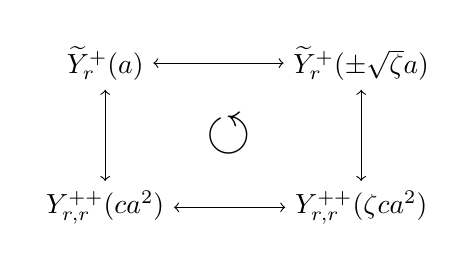
\begin{tikzpicture}
\matrix (m) [matrix of math nodes, row sep=1.5ex, column sep=2ex]
{
\tY_r^+(a)         &                     & \tY_r^+(\pm \sqrt{\zeta} a) \\
        & \text{\huge$\circlearrowleft$} &                             \\
Y_{r,r}^{++}(ca^2) &                     & Y_{r,r}^{++}(\zeta ca^2)    \\
};
\draw[<->] (m-1-1) -- (m-1-3);
\draw[<->] (m-1-3) -- (m-3-3);
\draw[<->] (m-3-3) -- (m-3-1);
\draw[<->] (m-3-1) -- (m-1-1);
\end{tikzpicture}
\end{figure}

This proves $\tY_r^+(a) \csim \tY_r^+(\pm \sqrt{\zeta}a)$ for $\zeta$ as above,
and since the diagram is commutative, there are no equivalences for other
values of the parameters than these. Hence
\[
P_1\left(\tY_r^+, \tY_r^+\right) = C\left(X^{2l}-1\right)
\]
with $l$ as above. The set $P_2\bigl(\tY_r^+, \tY_r^+\bigr)$ can now be
determined as in Section~\ref{ssec:computing_P2}. In fact it is easy to see
that
\[
P_2\left(\tY_r^+, \tY_r^+\right) = R\left(X^2-1\right) \,.
\]
We clearly have $(a, a) \in P_3\bigl(\tY_r^+, \tY_r^+\bigr)$ for
$a \in \R \setminus \{0\}$, and also
$(a, -a) \in P_3\bigl(\tY_r^+, \tY_r^+\bigr)$ if $r$ is odd. Let us now
consider $\tY_r^+(a)$ as a function in $x$ and $y$ over $\R^2$ and let the
parameter $a$ be positive. Then $\tY_r^+(a) = (x^2+y^2)^2+ax^r$ takes only
non-negative values whereas $\tY_r^+(-a) = (x^2+y^2)^2-ax^r$ attains also
negative values. Hence there is no real coordinate transformation which takes
$\tY_r^+(a)$ to $\tY_r^+(-a)$. The argument is similar for $a < 0$. To sum up,
we have
\[
P_3\left(\tY_r^+, \tY_r^+\right) =
\begin{cases}
R(X^2-1), &\text{if } r \text{ is odd}, \\
R(X-1),   &\text{if } r \text{ is even}.
\end{cases}
\]

\begin{remark}\label{rem:sufficient_sets_for_Yr}
For each even $r > 4$, let $\phi_r \in \Aut_{\C}(\C[[x,y]])$ be a coordinate
transformation which takes $\tY_r^+(a)$ to $\tY_r^+(-a)$. Then the degree of
either $\phi_r(x)$ or $\phi_r(y)$ must at least $\frac{r}{4}$. This shows that
there is no degree-bounded sufficient set of coordinate transformations for
$\bigl(\tY_r^+(a), \tY_r^+(a)\bigr)$ and for arbitrarily high $r$.
\end{remark}


\section{Results}\label{sec:results}

In this section we present the sets $P_1,P_2,P_3$ in table form for every
unimodal real singularity type up to corank 2.

\begin{theorem}\label{thm:X9}
The structure of the equivalence classes of the $X_9$ singularities is as shown
in Table~\ref{tab:X9_equivalences} where for $j = 1, \ldots, 6$ and
$\rho, \sigma \in \{1, i\}$, the function $f_j^{\rho, \sigma}$ is defined as
follows:
\begin{align*}
f_1^{\rho, \sigma}(a) &:= +\rho \sigma \cdot a \,, &
f_3^{\rho, \sigma}(a) &:= \frac{+2\sigma a+12\rho\sigma}{a-2\rho} \,, &
f_5^{\rho, \sigma}(a) &:= \frac{-2\sigma a+12\rho\sigma}{a+2\rho} \,, \\
f_2^{\rho, \sigma}(a) &:= -\rho \sigma \cdot a \,, &
f_4^{\rho, \sigma}(a) &:= \frac{+2\sigma a-12\rho\sigma}{a+2\rho} \,, &
f_6^{\rho, \sigma}(a) &:= \frac{-2\sigma a-12\rho\sigma}{a-2\rho} \,.
\end{align*}

Furthermore, we use the following notations:
\begin{align*}
\C'  &:= \C \setminus \{ -2, 2\} \,, &
\R'  &:= \R \setminus \{ -2, 2\} \,, &
\C'' &:= \C \setminus \{ -2i, 2i\} \,.
\end{align*}

\newcommand{\specialvrule}{\rule[-1.8ex]{0pt}{5ex}}
\begin{table}[htbp]
\centering
\caption{$P_1$, $P_2$ and $P_3$ for the $X_9$ singularities}
\label{tab:X9_equivalences}
\begin{tabular}{|c|c||c|c|c|}
\hline

$T_1$ & $T_2$ & $P_1(T_1, T_2)$ & $P_2(T_1, T_2)$ & $P_3(T_1, T_2)$ \\
\hline\hline

$X_9^{++}$ & $X_9^{++}$ &
\multirow{6}{*}{$\Gamma_{\C'}\left(f_1^{1,1}, \ldots, f_6^{1,1}\right)$} &
\multirow{6}{*}{$\Gamma_{\R'}\left(f_1^{1,1}, \ldots, f_6^{1,1}\right)$} &
\begin{tabular}[x]{@{}l@{}}
    $\phantom{\cup}\; \Gamma_{\R'}\left(f_1^{1,1}\right)$\specialvrule \\
    $\cup\; \Gamma_{\R^{>-2}}\left(f_5^{1,1}\right)$\specialvrule
\end{tabular}
\\ \cline{1-2}\cline{5-5}

$X_9^{--}$ & $X_9^{--}$ &&&
\begin{tabular}[x]{@{}l@{}}
    $\phantom{\cup}\; \Gamma_{\R'}\left(f_1^{1,1}\right)$\specialvrule \\
    $\cup\; \Gamma_{\R^{<2}}\left(f_3^{1,1}\right)$\specialvrule
\end{tabular}
\\ \cline{1-2}\cline{5-5}

$X_9^{++}$ & $X_9^{--}$ &&&
$\Gamma_{\R^{<-2}}\left(f_4^{1,1}\right)$\specialvrule
\\ \cline{1-2}\cline{5-5}

$X_9^{--}$ & $X_9^{++}$ &&&
$\Gamma_{\R^{>2}}\left(f_6^{1,1}\right)$\specialvrule
\\ \hline


$X_9^{+-}$ & $X_9^{+-}$ &
\multirow{4}{*}{$\Gamma_{\C''}\left(f_1^{i,i}, \ldots, f_6^{i,i}\right)$} &
\multirow{4}{*}{$\Gamma_{\R}\left(f_1^{1,1}, f_2^{1,1}\right)$} &
\multirow{4}{*}{$\Gamma_{\R}\left(f_1^{1,1}\right)$} \\ \cline{1-2}

$X_9^{-+}$ & $X_9^{-+}$ &&& \\ \cline{1-2}

$X_9^{+-}$ & $X_9^{-+}$ &&& \\ \cline{1-2}

$X_9^{-+}$ & $X_9^{+-}$ &&& \\ \hline


$X_9^{++}$ & $X_9^{+-}$ &
\multirow{4}{*}{$\Gamma_{\C'}\left(f_1^{1,i}, \ldots, f_6^{1,i}\right)$} &
\multirow{4}{*}{$\{(-6,0), (0,0), (6,0)\}$} &
\multirow{4}{*}{$\varnothing$} \\ \cline{1-2}

$X_9^{++}$ & $X_9^{-+}$ &&& \\ \cline{1-2}

$X_9^{--}$ & $X_9^{+-}$ &&& \\ \cline{1-2}

$X_9^{--}$ & $X_9^{-+}$ &&& \\ \hline


$X_9^{+-}$ & $X_9^{++}$ &
\multirow{4}{*}{$\Gamma_{\C''}\left(f_1^{i,1}, \ldots, f_6^{i,1}\right)$} &
\multirow{4}{*}{$\{(0,-6), (0,0), (0,6)\}$} &
\multirow{4}{*}{$\varnothing$} \\ \cline{1-2}

$X_9^{-+}$ & $X_9^{++}$ &&& \\ \cline{1-2}

$X_9^{+-}$ & $X_9^{--}$ &&& \\ \cline{1-2}

$X_9^{-+}$ & $X_9^{--}$ &&& \\ \hline
\end{tabular}
\end{table}

\end{theorem}


\begin{theorem}\label{thm:J10}
The structure of the equivalence classes of the $J_{10}$ singularities is as
shown in Table~\ref{tab:J10_equivalences} where for $j = 1, \ldots, 6$ and
$\rho, \sigma \in \{-1, +1\}$, the function $f_j^{\rho, \sigma}$ is defined as
follows:
\begin{align*}
f_1^{\rho, \sigma}(a) &:= +\sqrt{\rho \sigma} \cdot a \,, \\
f_2^{\rho, \sigma}(a) &:= -\sqrt{\rho \sigma} \cdot a \,, \\
f_3^{\rho, \sigma}(a)
&:= + \sqrt{\frac{-\rho \sigma (a^2-\rho \cdot 4) (a^2-\rho \cdot 9)
    + a (a^2-\rho \cdot 3) \sqrt{a^2-\rho \cdot 4}}{2(a^2-\rho \cdot 4)}}\,, \\
f_4^{\rho, \sigma}(a)
&:= - \sqrt{\frac{-\rho \sigma (a^2-\rho \cdot 4) (a^2-\rho \cdot 9)
    + a (a^2-\rho \cdot 3) \sqrt{a^2-\rho \cdot 4}}{2(a^2-\rho \cdot 4)}}\,, \\
f_5^{\rho, \sigma}(a)
&:= + \sqrt{\frac{-\rho \sigma (a^2-\rho \cdot 4) (a^2-\rho \cdot 9)
    - a (a^2-\rho \cdot 3) \sqrt{a^2-\rho \cdot 4}}{2(a^2-\rho \cdot 4)}}\,, \\
f_6^{\rho, \sigma}(a)
&:= - \sqrt{\frac{-\rho \sigma (a^2-\rho \cdot 4) (a^2-\rho \cdot 9)
    - a (a^2-\rho \cdot 3) \sqrt{a^2-\rho \cdot 4}}{2(a^2-\rho \cdot 4)}}\,.
\end{align*}

In each case, $\rho$ and $\sigma$ are given by
\begin{align*}
\rho &:=
\begin{cases}
    +1, &\text{if } T_1 = J_{10}^+ \,, \\
    -1, &\text{if } T_1 = J_{10}^- \,, \\
\end{cases}
&\sigma &:=
\begin{cases}
    +1, &\text{if } T_2 = J_{10}^+ \,, \\
    -1, &\text{if } T_2 = J_{10}^- \,. \\
\end{cases}
\end{align*}

Furthermore, we use the following notations:
\begin{align*}
\C'  &:= \C \setminus \{ -2, 2\} \,, &
\R'  &:= \R \setminus \{ -2, 2\} \,, \\
I_1 &:= \left] {\textstyle\frac{3}{\sqrt{2}}}, \infty \right[ \subset \R \,, &
I_2 &:= \left] 2, {\textstyle\frac{3}{\sqrt{2}}} \right[ \subset \R      \,, \\
I_3 &:= \left] {\textstyle-\frac{3}{\sqrt{2}}}, -2 \right[ \subset \R    \,, &
I_4 &:= \left] -\infty, {\textstyle-\frac{3}{\sqrt{2}}} \right[ \subset \R \,.
\end{align*}

\newcommand{\specialvrule}{\rule[-1.9ex]{0pt}{4.8ex}}
\begin{table}[htbp]
\centering
\caption{$P_1$, $P_2$ and $P_3$ for the $J_{10}$ singularities}
\label{tab:J10_equivalences}
\begin{tabular}{|c|c||c|c|c|}
\hline

$T_1$ & $T_2$ & $P_1(T_1, T_2)$ & $P_2(T_1, T_2)$ & $P_3(T_1, T_2)$ \\
\hline\hline

$J_{10}^+$ & $J_{10}^+$ &
$\Gamma_{\C'}\left(f_1^{\rho,\sigma}, \ldots, f_6^{\rho,\sigma}\right)$ &
\begin{tabular}[x]{@{}l@{}}
    $\phantom{\cup}\; \Gamma_{\R'}\left(f_1^{\rho,\sigma},
        f_2^{\rho,\sigma}\right)$ \\
    $\cup\; \Gamma_{\R^{>+2}}\left(f_3^{\rho,\sigma},
        f_4^{\rho,\sigma}\right)$ \\
    $\cup\; \Gamma_{\R^{<-2}}\left(f_5^{\rho,\sigma},
        f_6^{\rho,\sigma}\right)$ \\
    $\cup \left\{\left(0, \frac{-3}{\sqrt{2}}\right),
        \left(0, \frac{+3}{\sqrt{2}}\right)\right\}$\specialvrule \\
    $\cup \left\{\left(\frac{-3}{\sqrt{2}}, 0\right),
        \left(\frac{+3}{\sqrt{2}}, 0\right)\right\}$\specialvrule \\
\end{tabular} &
\begin{tabular}[x]{@{}l@{}}
    $\phantom{\cup}\; \Gamma_{\R'}\left(f_1^{\rho,\sigma}\right)$ \\
    $\cup\; \Gamma_{\R^{>+2}}\left(f_4^{\rho,\sigma}\right)$ \\
    $\cup\; \Gamma_{\R^{<-2}}\left(f_5^{\rho,\sigma}\right)$ \\
\end{tabular} \\
\hline

$J_{10}^-$ & $J_{10}^-$ &
$\Gamma_{\C}\left(f_1^{\rho,\sigma}, \ldots, f_6^{\rho,\sigma}\right)$ &
$\Gamma_{\R}\left(f_1^{\rho,\sigma}, f_2^{\rho,\sigma}\right)$ &
$\Gamma_{\R}\left(f_1^{\rho,\sigma}\right)$ \\
\hline

$J_{10}^+$ & $J_{10}^-$ &
$\Gamma_{\C'}\left(f_1^{\rho,\sigma}, \ldots, f_6^{\rho,\sigma}\right)$ &
\begin{tabular}[x]{@{}l@{}}
    $\phantom{\cup}\; \{(0, 0)\}$ \\
    $\cup\; \Gamma_{\R^{>+2}}\left(f_3^{\rho,\sigma},
        f_4^{\rho,\sigma}\right)$ \\
    $\cup\; \Gamma_{\R^{<-2}}\left(f_5^{\rho,\sigma},
        f_6^{\rho,\sigma}\right)$ \\
\end{tabular} &
\begin{tabular}[x]{@{}l@{}}
    $\phantom{\cup}\; \Gamma_{I_1} \left(f_3^{\rho,\sigma}\right)$ \\
    $\cup\; \Gamma_{I_2} \left(f_4^{\rho,\sigma}\right)$ \\
    $\cup\; \Gamma_{I_3} \left(f_5^{\rho,\sigma}\right)$ \\
    $\cup\; \Gamma_{I_4} \left(f_6^{\rho,\sigma}\right)$ \\
    $\cup \left\{\left(\frac{-3}{\sqrt{2}}, 0\right),
        \left(\frac{+3}{\sqrt{2}}, 0\right)\right\}$\specialvrule \\
\end{tabular} \\
\hline

$J_{10}^-$ & $J_{10}^+$ &
$\Gamma_{\C}\left(f_1^{\rho,\sigma}, \ldots, f_6^{\rho,\sigma}\right)$ &
\begin{tabular}[x]{@{}l@{}}
    $\phantom{\cup}\; \{(0, 0)\}$ \\
    $\cup\; \Gamma_{\R}\left(f_3^{\rho,\sigma}, \ldots,
        f_6^{\rho,\sigma}\right)$ \\
\end{tabular} &
\begin{tabular}[x]{@{}l@{}}
    $\phantom{\cup}\; \Gamma_{\R^{>0}}\left(f_3^{\rho,\sigma},
        f_6^{\rho,\sigma}\right)$ \\
    $\cup\; \Gamma_{\R^{<0}}\left(f_4^{\rho,\sigma},
        f_5^{\rho,\sigma}\right)$ \\
    $\cup \left\{\left(0, \frac{-3}{\sqrt{2}}\right),
        \left(0, \frac{+3}{\sqrt{2}}\right)\right\}$\specialvrule \\
\end{tabular} \\
\hline

\end{tabular}
\end{table}

\end{theorem}


\begin{theorem}
The structure of the equivalence classes of the $J_{10+k}$
singularities is as shown in Table~\ref{tab:J10+k_equivalences} where in each
case, $l$ and $s$ are given by
\begin{align*}
l &:= \frac{6}{\gcd(6,k)}, \text{ and} \\
s &:=
\begin{cases}
  +1, &\text{if } k \equiv 2 \pmod{4}, \\
  -1, &\text{else.}
\end{cases}
\end{align*}

\begin{table}[htbp]
\centering
\caption{$P_1$, $P_2$ and $P_3$ for the $J_{10+k}$ singularities}
\label{tab:J10+k_equivalences}
\begin{tabular}{|c|c||c|c|c|}
\hline

$T_1$ & $T_2$ & $P_1(T_1, T_2)$ & $P_2(T_1, T_2)$ & $P_3(T_1, T_2)$ \\
\hline\hline

$J_{10+k}^+$ & $J_{10+k}^+$ &
\multirow{2}{*}{$C(X^l-1)$} &
\multirow{2}{*}{$R(X^l-1)$} &
\multirow{2}{*}{$R(X^l-1)$} \\
\cline{1-2}

$J_{10+k}^-$ & $J_{10+k}^-$ &&& \\
\hline

$J_{10+k}^+$ & $J_{10+k}^-$ &
\multirow{2}{*}{$C(X^l-s)$} &
\multirow{2}{*}{$R(X^l-s)$} &
\multirow{2}{*}{$\varnothing$} \\
\cline{1-2}

$J_{10+k}^-$ & $J_{10+k}^+$ &&& \\
\hline

\end{tabular}
\end{table}

\end{theorem}


\begin{theorem}
The structure of the equivalence classes of the $X_{9+k}$
singularities is as shown in Table~\ref{tab:X9+k_equivalences} where in each
case, $l$ and $s$ are given by
\begin{align*}
l &:= \frac{4}{\gcd(4,k)}, \text{ and} \\
s &:=
\begin{cases}
  +1, &\text{if } k \equiv 4 \pmod{8}, \\
  -1, &\text{else.}
\end{cases}
\end{align*}

\begin{table}[htbp]
\centering
\caption{$P_1$, $P_2$ and $P_3$ for the $X_{9+k}$ singularities}
\label{tab:X9+k_equivalences}
\begin{tabular}{|c|c||c|c|c|}
\hline

$T_1$ & $T_2$ & $P_1(T_1, T_2)$ & $P_2(T_1, T_2)$ & $P_3(T_1, T_2)$ \\
\hline\hline

$X_{9+k}^{++}$ & $X_{9+k}^{++}$ &
\multirow{4}{*}{$C(X^l-1)$} &
\multirow{4}{*}{$R(X^l-1)$} &
\multirow{4}{*}{$R(X^{k+1}-1)$} \\
\cline{1-2}

$X_{9+k}^{+-}$ & $X_{9+k}^{+-}$ &&& \\ \cline{1-2}
$X_{9+k}^{-+}$ & $X_{9+k}^{-+}$ &&& \\ \cline{1-2}
$X_{9+k}^{--}$ & $X_{9+k}^{--}$ &&& \\ \hline


$X_{9+k}^{++}$ & $X_{9+k}^{+-}$ &
\multirow{4}{*}{$C(X^l-1)$} &
\multirow{4}{*}{$R(X^l-1)$} &
\multirow{4}{*}{$\varnothing$} \\
\cline{1-2}

$X_{9+k}^{+-}$ & $X_{9+k}^{++}$ &&& \\ \cline{1-2}
$X_{9+k}^{-+}$ & $X_{9+k}^{--}$ &&& \\ \cline{1-2}
$X_{9+k}^{--}$ & $X_{9+k}^{-+}$ &&& \\ \hline


$X_{9+k}^{++}$ & $X_{9+k}^{-+}$ &
\multirow{4}{*}{$C(X^l-s)$} &
\multirow{4}{*}{$R(X^l-s)$} &
\multirow{4}{*}{$\varnothing$} \\
\cline{1-2}

$X_{9+k}^{+-}$ & $X_{9+k}^{--}$ &&& \\ \cline{1-2}
$X_{9+k}^{-+}$ & $X_{9+k}^{++}$ &&& \\ \cline{1-2}
$X_{9+k}^{--}$ & $X_{9+k}^{+-}$ &&& \\ \hline


$X_{9+k}^{++}$ & $X_{9+k}^{--}$ &
\multirow{4}{*}{$C(X^l-s)$} &
\multirow{4}{*}{$R(X^l-s)$} &
\multirow{4}{*}{$\varnothing$} \\
\cline{1-2}

$X_{9+k}^{+-}$ & $X_{9+k}^{-+}$ &&& \\ \cline{1-2}
$X_{9+k}^{-+}$ & $X_{9+k}^{+-}$ &&& \\ \cline{1-2}
$X_{9+k}^{--}$ & $X_{9+k}^{++}$ &&& \\ \hline

\end{tabular}
\end{table}

\end{theorem}


\begin{theorem}\label{thm:Yrs}
The structure of the equivalence classes of the $Y_{r,s}$ singularities is as
shown in Table~\ref{tab:Yrs_equivalences} where in each case, $l$, $s_1$ and
$s_2$ are given by
\begin{align*}
l &:= \frac{r}{\gcd(r,s)} \cdot \gcd(2, r+1, s+1) \,, \\
s_1 &:=
\begin{cases}
  +1, &\text{if } r \equiv 0 \pmod{4} \text{ or } s \equiv 0 \pmod{4}, \\
  -1, &\text{else,}
\end{cases} \\
s_2 &:=
\begin{cases}
  +1, &\text{if } r \not\equiv 0 \pmod{2}
      \text{ or } \frac{s}{\gcd(r,s)} \equiv 0 \pmod{2}, \\
  -1, &\text{else.}
\end{cases}
\end{align*}

In the special case where $r = s$, additional equivalences occur. They are
listed in Table~\ref{tab:Yrr_equivalences}.

\begin{table}[htbp]
\centering
\caption{$P_1$, $P_2$ and $P_3$ for the $Y_{r,s}$ singularities}
\label{tab:Yrs_equivalences}
\begin{tabular}{|c|c||c|c|c|}
\hline

$T_1$ & $T_2$ & $P_1(T_1, T_2)$ & $P_2(T_1, T_2)$ & $P_3(T_1, T_2)$ \\
\hline\hline

$Y_{r,s}^{++}$ & $Y_{r,s}^{++}$ &
\multirow{4}{*}{$C(X^l-1)$} &
\multirow{4}{*}{$R(X^l-1)$} &
\multirow{4}{*}{$R(X^{s+1}-1)$}
\\ \cline{1-2}

$Y_{r,s}^{-+}$ & $Y_{r,s}^{-+}$ &&&
\\ \cline{1-2}

$Y_{r,s}^{+-}$ & $Y_{r,s}^{+-}$ &&&
\\ \cline{1-2}

$Y_{r,s}^{--}$ & $Y_{r,s}^{--}$ &&&
\\ \hline


$Y_{r,s}^{++}$ & $Y_{r,s}^{-+}$ &
\multirow{4}{*}{$C(X^l-s_1)$} &
\multirow{4}{*}{$R(X^l-s_1)$} &
\multirow{4}{*}{$\varnothing$}
\\ \cline{1-2}

$Y_{r,s}^{-+}$ & $Y_{r,s}^{++}$ &&&
\\ \cline{1-2}

$Y_{r,s}^{+-}$ & $Y_{r,s}^{--}$ &&&
\\ \cline{1-2}

$Y_{r,s}^{--}$ & $Y_{r,s}^{+-}$ &&&
\\ \hline


$Y_{r,s}^{++}$ & $Y_{r,s}^{+-}$ &
\multirow{4}{*}{$C(X^l-s_2)$} &
\multirow{4}{*}{$R(X^l-s_2)$} &
\multirow{4}{*}{$\begin{cases}
  R(X^l-s_2),  &\text{if } r \not\equiv 0 \pmod{2} \\
  \varnothing, &\text{if } r \equiv 0 \pmod{2}
\end{cases}$}
\\ \cline{1-2}

$Y_{r,s}^{-+}$ & $Y_{r,s}^{--}$ &&&
\\ \cline{1-2}

$Y_{r,s}^{+-}$ & $Y_{r,s}^{++}$ &&&
\\ \cline{1-2}

$Y_{r,s}^{--}$ & $Y_{r,s}^{-+}$ &&&
\\ \hline


$Y_{r,s}^{++}$ & $Y_{r,s}^{--}$ &
\multirow{4}{*}{$C(X^l-s_1 s_2)$} &
\multirow{4}{*}{$R(X^l-s_1 s_2)$} &
\multirow{4}{*}{$\varnothing$}
\\ \cline{1-2}

$Y_{r,s}^{-+}$ & $Y_{r,s}^{+-}$ &&&
\\ \cline{1-2}

$Y_{r,s}^{+-}$ & $Y_{r,s}^{-+}$ &&&
\\ \cline{1-2}

$Y_{r,s}^{--}$ & $Y_{r,s}^{++}$ &&&
\\ \hline

\end{tabular}
\end{table}

\begin{table}[htbp]
\centering
\caption{Additional equivalences for the $Y_{r,s}$ singularities in the
special case $r = s$}
\label{tab:Yrr_equivalences}
\begin{tabular}{|c|c||c|}
\hline

$T_1$ & $T_2$ & $P_3(T_1, T_2)$ \\
\hline\hline

$Y_{r,s}^{++}$ & $Y_{r,s}^{+-}$ &
\multirow{2}{*}{$\begin{cases}
  R(X+1),      &\!\text{if } r \equiv 0 \pmod{2} \text{ and } a < 0 \\
  \varnothing, &else
\end{cases}$}
\\ \cline{1-2}

$Y_{r,s}^{-+}$ & $Y_{r,s}^{--}$ &
\\ \hline

$Y_{r,s}^{+-}$ & $Y_{r,s}^{++}$ &
\multirow{2}{*}{$\begin{cases}
  R(X+1),      &\!\text{if } r \equiv 0 \pmod{2} \text{ and } a > 0 \\
  \varnothing, &else
\end{cases}$}
\\ \cline{1-2}

$Y_{r,s}^{--}$ & $Y_{r,s}^{-+}$ &
\\ \hline

\end{tabular}
\end{table}

\end{theorem}


\begin{theorem}
The structure of the equivalence classes of the $\tY_r$ singularities is as
shown in Table~\ref{tab:tYr_equivalences} where in each case, $l$ and $s$ are
given by
\begin{align*}
l &:= 2\cdot{\gcd(2, r+1)}, \text{ and} \\
s &:=
\begin{cases}
  +1, &\text{if } r \equiv 0 \pmod{4}, \\
  -1, &\text{else.}
\end{cases}
\end{align*}

\begin{table}[htbp]
\centering
\caption{$P_1$, $P_2$ and $P_3$ for the $\tY_r$ singularities}
\label{tab:tYr_equivalences}
\begin{tabular}{|c|c||c|c|c|}
\hline

$T_1$ & $T_2$ & $P_1(T_1, T_2)$ & $P_2(T_1, T_2)$ & $P_3(T_1, T_2)$ \\
\hline\hline

$\tY_r^+$ & $\tY_r^+$ &
\multirow{2}{*}{$C(X^l-1)$} &
\multirow{2}{*}{$R(X^2-1)$} &
\multirow{2}{*}{$\begin{cases}
  R(X^2-1), &\text{if } r \equiv 1 \pmod{2} \\
  R(X-1),   &\text{if } r \equiv 0 \pmod{2}
\end{cases}$} \\
\cline{1-2}

$\tY_r^-$ & $\tY_r^-$ &
&
&
\\
\hline

$\tY_r^+$ & $\tY_r^-$ &
\multirow{2}{*}{$C(X^l-s)$} &
\multirow{2}{*}{$R(X^2-s)$} &
\multirow{2}{*}{$\varnothing$} \\
\cline{1-2}

$\tY_r^-$ & $\tY_r^+$ &
&
&
\\
\hline

\end{tabular}
\end{table}

\end{theorem}


\begin{theorem}
The structure of the equivalence classes of the exceptional unimodal
singularities is as shown in Table~\ref{tab:exceptional_equivalences}.

\begin{table}[htbp]
\centering
\caption{$P_1$, $P_2$ and $P_3$ for the exceptional unimodal singularities}
\label{tab:exceptional_equivalences}
\begin{tabular}{|c|c||c|c|c|}
\hline
$T_1$ & $T_2$ & $P_1(T_1, T_2)$ & $P_2(T_1, T_2)$ & $P_3(T_1, T_2)$ \\
\hline\hline
$E_{12}$   & $E_{12}$   & $C(X^{21}-1)$ & $R(X-1)$      & $R(X-1)$ \\
\hline
$E_{13}$   & $E_{13}$   & $C(X^{15}-1)$ & $R(X-1)$      & $R(X-1)$ \\
\hline
$E_{14}^+$ & $E_{14}^+$ & $C(X^{12}-1)$ & $R(X^2-1)$    & $R(X-1)$ \\
\hline
$E_{14}^-$ & $E_{14}^-$ & $C(X^{12}-1)$ & $R(X^2-1)$    & $R(X-1)$ \\
\hline
$E_{14}^+$ & $E_{14}^-$ & $C(X^{12}+1)$ & $\varnothing$ & $\varnothing$ \\
\hline
$E_{14}^-$ & $E_{14}^+$ & $C(X^{12}+1)$ & $\varnothing$ & $\varnothing$ \\
\hline
$Z_{11}$   & $Z_{11}$   & $C(X^{15}-1)$ & $R(X-1)$      & $R(X-1)$ \\
\hline
$Z_{12}$   & $Z_{12}$   & $C(X^{11}-1)$ & $R(X-1)$      & $R(X-1)$ \\
\hline
$Z_{13}^+$ & $Z_{13}^+$ & $C(X^9-1)$    & $R(X-1)$      & $R(X-1)$ \\
\hline
$Z_{13}^-$ & $Z_{13}^-$ & $C(X^9-1)$    & $R(X-1)$      & $R(X-1)$ \\
\hline
$Z_{13}^+$ & $Z_{13}^-$ & $C(X^9+1)$    & $R(X+1)$      & $\varnothing$ \\
\hline
$Z_{13}^-$ & $Z_{13}^+$ & $C(X^9+1)$    & $R(X+1)$      & $\varnothing$ \\
\hline
$W_{12}^+$ & $W_{12}^+$ & $C(X^{10}-1)$ & $R(X^2-1)$    & $R(X-1)$ \\
\hline
$W_{12}^-$ & $W_{12}^-$ & $C(X^{10}-1)$ & $R(X^2-1)$    & $R(X-1)$ \\
\hline
$W_{12}^+$ & $W_{12}^-$ & $C(X^{10}+1)$ & $\varnothing$ & $\varnothing$ \\
\hline
$W_{12}^-$ & $W_{12}^+$ & $C(X^{10}+1)$ & $\varnothing$ & $\varnothing$ \\
\hline
$W_{13}^+$ & $W_{13}^+$ & $C(X^8-1)$    & $R(X^2-1)$    & $R(X-1)$ \\
\hline
$W_{13}^-$ & $W_{13}^-$ & $C(X^8-1)$    & $R(X^2-1)$    & $R(X-1)$ \\
\hline
$W_{13}^+$ & $W_{13}^-$ & $C(X^8+1)$    & $\varnothing$ & $\varnothing$ \\
\hline
$W_{13}^-$ & $W_{13}^+$ & $C(X^8+1)$    & $\varnothing$ & $\varnothing$ \\
\hline
\end{tabular}
\end{table}

\end{theorem}


\section{Interpretation of the Results}

\begin{remark}
Note that the $J_{10}^-$ normal form is redundant. Also note that although
$J_{10}^+$ covers the $\mu$-constant stratum in the real case $J_{10}^-$ does
not.
\end{remark}


\section{Acknowledgements}

We would like to thank Claus Fieker, Gert-Martin Greuel, and Gerhard Pfister
for many fruitful discussions.


\clearpage

\begin{thebibliography}{99}

\bibitem[{Arnold(1974)}]{A1974}
Arnold, V.I., 1974.
Normal forms of functions in neighbourhoods of degenerate critical points.
Russ. Math. Surv. 29(2), 10-50.

\bibitem[{Arnold et al.(1985)}]{AVG1985}
Arnold, V.I., Gusein-Zade, S.M., Varchenko, A.N., 1985.
Singularities of Differential Maps, Vol.~I.
Birkh\"auser, Boston.

\bibitem[{Decker et al.(2012a)}]{DGPS}
Decker, W., Greuel, G.-M., Pfister, G., Sch{\"o}nemann, H., 2012.
{\sc Singular} {3-1-6} -- {A} computer algebra system for polynomial
computations.
\url{http://www.singular.uni-kl.de}.

\bibitem[{Decker et al.(2012b)}]{primdec}
Decker, W., Laplagne, S., Pfister, G., Sch\"onemann, H., 2012.
{\tt primdec.lib}. {A} {\sc Singular} {3-1-6} library for primary decomposition
and radicals of ideals.

\bibitem[{Greuel et al.(2007)}]{GLS2007}
Greuel, G.-M., Lossen, C., Shustin, E., 2007.
Introduction to Singularities and Deformations.
Springer, Berlin.

\bibitem[{Greuel and Pfister(2008)}]{GP2008}
Greuel, G.-M., Pfister, G., 2008.
A Singular Introduction to Commutative Algebra, second ed.
Springer, Berlin.

\bibitem[{Kr\"uger(2012)}]{classify}
Kr\"uger, K., 2012.
{\tt classify.lib}. {A} {\sc Singular} {3-1-6} library for classifying isolated
hypersurface singularities w.r.t.\@ right equivalence, based on the
determinator of singularities by V.I. Arnold.

\bibitem[{Marais and Steenpa\ss(2012)}]{realclassify}
Marais, M.S., Steenpa\ss, A., 2012.
{\tt realclassify.lib}. {A} {\sc Singular} {3-1-6} library for classifying
isolated hypersurface singularities over the reals w.r.t.\@ right equivalence.

\bibitem[{Marais and Steenpa\ss(2013)}]{MS2013}
Marais, M.S., Steenpa\ss, A., 2013.
The Classification of Real Singularities Using \Singular{}. Part I: Splitting
Lemma and Simple Singularities.

\bibitem[{Montes and Sch\"onemann(2012)}]{grobcov}
Montes, A., Sch\"onemann, H., 2012.
{\tt grobcov.lib}. {A} {\sc Singular} {3-1-6} library for Gr\"obner covers of
parametric ideals.

\bibitem[{Siersma(1974)}]{Siersma}
Siersma, D., 1974.
Classification and Deformation of Singularities.
Dissertation, University of Amsterdam.

\end{thebibliography}

\end{document}
